\documentclass[aspectratio=169,12pt]{beamer}
\usepackage[utf8]{inputenc}
\usepackage{amsmath, amssymb}
\usepackage{booktabs}
\usepackage{hyperref}
\usepackage{listings}
\usepackage{tikz}
\usetikzlibrary{arrows.meta, positioning, shapes.geometric, calc}

\usetheme{Madrid}
% Show slide number as "current/total" in the footer
\setbeamertemplate{footline}{%
  \leavevmode\hbox{\begin{beamercolorbox}[wd=\paperwidth,ht=2.25ex,dp=1ex,center]{author in head/foot}%
    \usebeamerfont{author in head/foot}\insertframenumber/\inserttotalframenumber
  \end{beamercolorbox}}%
  \vskip0pt%
}
\setbeamertemplate{navigation symbols}{}

\title{Computer Structure -- Cache Memory}
\author{Based on slides by Lihu Rappoport}
\date{Technion CSL}

\begin{document}

\begin{frame}
  \titlepage
\end{frame}

% --- Overview
\begin{frame}{Processor--Memory Gap (summary)}
\begin{itemize}
  \item CPU performance has improved much faster than DRAM latency/bandwidth.
  \item The performance gap has grown roughly $\sim 50\%$/year historically.
  \item Motivation: hide long memory access times from the CPU.
\end{itemize}
\end{frame}

\begin{frame}{Memory Trade-Offs}
\begin{itemize}
  \item Large (dense) memories are \textbf{slow}
  \item Fast memories are \textbf{small}, expensive and consume high power
  \item Goal: give the processor the feeling that it has a memory which is large (dense), fast, consumes low power, and cheap
  \item Solution: a hierarchy of memories
\end{itemize}

\vspace{0.3cm}
\begin{center}
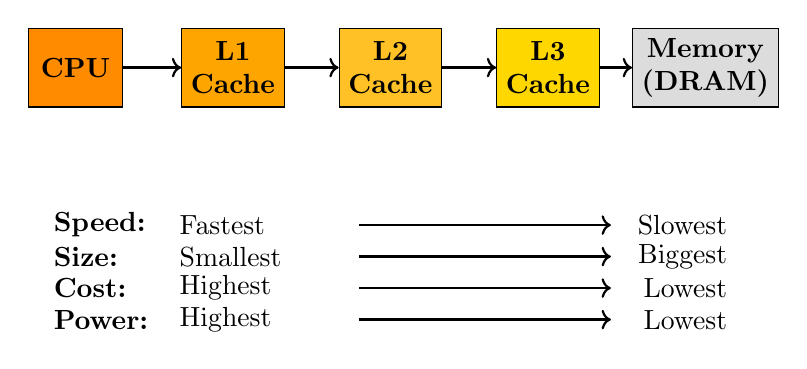
\begin{tikzpicture}[scale=0.8]
  % Define colors for the hierarchy
  \definecolor{cpucolor}{RGB}{255,140,0}      % Orange
  \definecolor{l1color}{RGB}{255,165,0}       % Orange
  \definecolor{l2color}{RGB}{255,193,37}      % Yellow-orange
  \definecolor{l3color}{RGB}{255,215,0}       % Gold
  \definecolor{memcolor}{RGB}{220,220,220}    % Light gray
  
  % Memory hierarchy boxes
  \node[rectangle, draw, fill=cpucolor, minimum width=1.2cm, minimum height=1cm, align=center, font=\bfseries] (cpu) at (0,0) {CPU};
  \node[rectangle, draw, fill=l1color, minimum width=1.2cm, minimum height=1cm, align=center, font=\bfseries] (l1) at (2.5,0) {L1\\Cache};
  \node[rectangle, draw, fill=l2color, minimum width=1.2cm, minimum height=1cm, align=center, font=\bfseries] (l2) at (5,0) {L2\\Cache};
  \node[rectangle, draw, fill=l3color, minimum width=1.2cm, minimum height=1cm, align=center, font=\bfseries] (l3) at (7.5,0) {L3\\Cache};
  \node[rectangle, draw, fill=memcolor, minimum width=1.2cm, minimum height=1cm, align=center, font=\bfseries] (mem) at (10,0) {Memory\\(DRAM)};
  
  % Arrows between boxes
  \draw[->, thick] (cpu.east) -- (l1.west);
  \draw[->, thick] (l1.east) -- (l2.west);
  \draw[->, thick] (l2.east) -- (l3.west);
  \draw[->, thick] (l3.east) -- (mem.west);
  
  % Characteristics table below
  \node[anchor=west, font=\bfseries] at (-0.5,-2.5) {Speed:};
  \node[anchor=west] at (1.5,-2.5) {Fastest};
  \draw[->, thick] (4.5,-2.5) -- (8.5,-2.5);
  \node[anchor=east] at (10.5,-2.5) {Slowest};
  
  \node[anchor=west, font=\bfseries] at (-0.5,-3) {Size:};
  \node[anchor=west] at (1.5,-3) {Smallest};
  \draw[->, thick] (4.5,-3) -- (8.5,-3);
  \node[anchor=east] at (10.5,-3) {Biggest};
  
  \node[anchor=west, font=\bfseries] at (-0.5,-3.5) {Cost:};
  \node[anchor=west] at (1.5,-3.5) {Highest};
  \draw[->, thick] (4.5,-3.5) -- (8.5,-3.5);
  \node[anchor=east] at (10.5,-3.5) {Lowest};
  
  \node[anchor=west, font=\bfseries] at (-0.5,-4) {Power:};
  \node[anchor=west] at (1.5,-4) {Highest};
  \draw[->, thick] (4.5,-4) -- (8.5,-4);
  \node[anchor=east] at (10.5,-4) {Lowest};
\end{tikzpicture}
\end{center}
\end{frame}

\begin{frame}{Why Hierarchy Works}
\begin{itemize}
  \item \textbf{Temporal Locality (Locality in Time):}
  \begin{itemize}
    \item If an item is referenced, it will tend to be referenced again soon
    \item Example: code and variables in loops
  \end{itemize}
  $\Rightarrow$ \textbf{Keep recently accessed data closer to the processor}
  
  \vspace{0.5cm}
  
  \item \textbf{Spatial Locality (Locality in Space):}
  \begin{itemize}
    \item If an item is referenced, nearby items tend to be referenced soon
    \item Example: scanning an array
  \end{itemize}
  $\Rightarrow$ \textbf{Move contiguous blocks closer to the processor}
  
  \vspace{0.5cm}
  
  \item \textbf{Locality + smaller HW is faster + Amdahl's law}\\
  $\Rightarrow$ \textbf{memory hierarchy}
\end{itemize}
\end{frame}

\begin{frame}{Memory Hierarchy: Terminology}
\begin{itemize}
  \item \textbf{For each memory level, define the following:}
  \begin{itemize}
    \item \textcolor{green!60!black}{\textbf{Hit:}} data at the requested address is available in the cache level
    \item \textcolor{green!60!black}{\textbf{Miss:}} data at the requested address is not available in the cache level
    \item \textcolor{green!60!black}{\textbf{Hit Rate:}} the fraction of accesses that hit in that cache level
    \begin{itemize}
      \item For L1 cache: \#L1 hits / \#data accesses in the program
      \item For L2 cache: \#L2 hits / \#L1 misses
    \end{itemize}
    \item \textcolor{green!60!black}{\textbf{Hit Time:}} time from data request until data received when hitting in the cache level; includes the time to determine hit/miss
    \item \textcolor{green!60!black}{\textbf{Miss Rate}} = $1 - (\text{Hit Rate})$
    \item \textcolor{green!60!black}{\textbf{Miss Penalty:}} Time to replace a block in the upper level + Time to deliver the block to the processor
  \end{itemize}
  
  \vspace{0.3cm}
  
  \item \textbf{Average memory-access time =}\\
  \hspace{1cm} $t_{\text{effective}} = (\text{Hit time} \times \text{Hit Rate}) + (\text{Miss Time} \times \text{Miss rate})$\\
  \hspace{2.2cm} $= (\text{Hit time} \times \text{Hit Rate}) + (\text{Miss Time} \times (1-\text{Hit rate}))$
  \begin{itemize}
    \item If hit rate is close to 1, $t_{\text{effective}}$ is close to hit time
  \end{itemize}
\end{itemize}
\end{frame}

\begin{frame}{Effective Memory Access Time}
\begin{itemize}
  \item \textbf{Cache -- holds a subset of the memory}
  \begin{itemize}
    \item Hopefully -- the subset being used now
  \end{itemize}
  
  \item \textbf{Effective memory access time}
  \begin{itemize}
    \item $t_{\text{effective}} = (t_{\text{cache}} \times \text{Hit Rate}) + (t_{\text{mem}} \times (1 - \text{Hit rate}))$
    \item $t_{\text{mem}}$ includes the time it takes to detect a cache miss
  \end{itemize}
  
  \item \textbf{Example}
  \begin{itemize}
    \item Assume $t_{\text{cache}} = 10$ nsec and $t_{\text{mem}} = 100$ nsec
  \end{itemize}
\end{itemize}

\begin{center}
\begin{tabular}{c|c|l}
\textbf{Hit Rate} & \textbf{$t_{\text{eff}}$ (nsec)} & \textbf{Computation} \\
\hline
0 & 100 & $(0.0 \times 10) + (1.0 \times 100)$ \\
50 & 55 & $(0.5 \times 10) + (0.5 \times 100)$ \\
90 & 19 & $(0.9 \times 10) + (0.1 \times 100)$ \\
99 & 10.9 & $(0.99 \times 10) + (0.01 \times 100)$ \\
99.9 & 10.1 & $(0.999 \times 10) + (0.001 \times 100)$ \\
\end{tabular}
\end{center}

\begin{itemize}
  \item $t_{\text{mem}}/t_{\text{cache}}$ ratio increases $\Rightarrow$ hit-rate is more important
\end{itemize}
\end{frame}

\begin{frame}{Cache: Main Idea}
\begin{columns}[T]
\begin{column}{0.65\textwidth}
\begin{itemize}
  \item \textcolor{blue}{\textbf{The cache holds a small part of the memory}}
  \begin{itemize}
    \item Need to map parts of memory into the cache
  \end{itemize}
  
  \item \textcolor{blue}{\textbf{Memory is (logically) partitioned into blocks}}
  \begin{itemize}
    \item Typical block size is 32 or 64 bytes
    \item Blocks are aligned
  \end{itemize}
  
  \item \textcolor{blue}{\textbf{The cache is partitioned into cache lines}}
  \begin{itemize}
    \item Each cache line holds a memory block
    \item Only a subset of the memory blocks are mapped to the cache at a given time
    \item The cache views an address as:
  \end{itemize}
\end{itemize}

% Address format at the bottom of text
\begin{center}
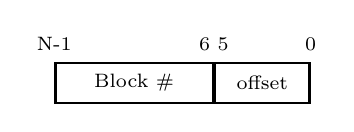
\begin{tikzpicture}[
    scale=1,
    box/.style={font=\scriptsize, minimum height=0.5cm, draw, thick, align=center, inner sep=2pt}
]

  % Bottom row (actual fields, in boxes)
  \node[box, minimum width=2.0cm] (block) {Block \#};
  \node[box, minimum width=1.2cm, right=0cm of block] (offset) {offset};

  % Numbers above (plain text only, no boxes)
  \node[font=\scriptsize, above=0.03cm of block.north west, anchor=south] {N-1};
  \node[font=\scriptsize, above=0.03cm of block.north east, anchor=south] {6 5};
  \node[font=\scriptsize, above=0.03cm of offset.north east, anchor=south] {0};

\end{tikzpicture}
\end{center}
\end{column}

\begin{column}{0.35\textwidth}
\centering
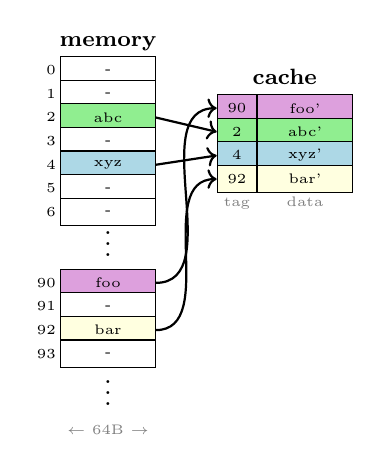
\begin{tikzpicture}[scale=0.6]
  % Define colors
  \definecolor{lightblue}{RGB}{173,216,230}
  \definecolor{lightgreen}{RGB}{144,238,144}
  \definecolor{lightyellow}{RGB}{255,255,224}
  \definecolor{lightpurple}{RGB}{221,160,221}
  
  % Memory blocks (with data)
  \foreach \i/\y/\color/\data in {
    0/4/white/-, 
    1/3.5/white/-, 
    2/3/lightgreen/abc, 
    3/2.5/white/-, 
    4/2/lightblue/xyz, 
    5/1.5/white/-, 
    6/1/white/-
  } {
    \node[anchor=east, font=\tiny] at (0.3, \y) {\i};
    \node[font=\tiny, inner sep=0.1pt, rectangle, draw, minimum width=1.2cm, minimum height=0.35cm, fill=\color] (mem\i) at (1.2, \y) {\data};
  }
  
  % Memory title (positioned above the memory blocks)
  \node[font=\footnotesize\bfseries, anchor=south] at (1.2, 4.2) {memory};
  
  % Dots to indicate gap
  \node at (1.2, 0.5) {$\vdots$};
  
  % Bottom memory blocks (with data)
  \foreach \i/\y/\color/\data in {
    90/-0.5/lightpurple/foo, 
    91/-1/white/-, 
    92/-1.5/lightyellow/bar, 
    93/-2/white/-
  } {
    \node[anchor=east, font=\tiny] at (0.3, \y) {\i};
    \node[font=\tiny, inner sep=0.1pt, rectangle, draw, minimum width=1.2cm, minimum height=0.35cm, fill=\color] (mem\i) at (1.2, \y) {\data};
  }
  
  % More dots
  \node[anchor=north] at (mem93) (dots) {$\vdots$};
  
  % 64B width indicator at bottom of memory
  \node[gray, font=\tiny,anchor=north] at (dots.south) {$\leftarrow$ 64B $\rightarrow$};
 
  % Cache entries (tag + data boxes)
  % Each cache line has a tag box (block number) and a data box positioned relative to tag
\foreach \block/\y/\color/\data in {
    90/3.5/lightpurple/foo',
    2/3/lightgreen/abc',
    4/2.5/lightblue/xyz',
    92/2/lightyellow/bar'
  } {
    % Tag box
    \node[font=\tiny, rectangle, draw, minimum width=0.5cm, minimum height=0.35cm,
          fill=\color, anchor=north west, inner sep=0.1pt] (tag\block) at (3.5,\y) {\block};

    % Data box (aligned exactly with tag box)
    \node[font=\tiny, rectangle, draw, minimum width=1.2cm, minimum height=0.35cm,
          fill=\color, anchor=north west, inner sep=0.1pt] (data\block) at (tag\block.north east) {\data};
  }
  
  % Cache title (calculated as middle between tag90.west and data90.east)
  \node[font=\footnotesize\bfseries, anchor=south] at ($(tag90.north west)!0.5!(data90.north east)$) {cache};
  
  % Labels for cache structure at the bottom
  \node[font=\tiny, gray, anchor=north,
        text height=0.25ex, text depth=0.25ex] 
        at (tag92.south) (tag_label) {tag};

  \node[font=\tiny, gray,
        text height=0.25ex, text depth=0.25ex] 
        at (data92 |- tag_label) {data};
  
  % Arrows from memory to cache (pointing to tag boxes)
  \draw[->, thick] (mem2.east) -- (tag2.west);
  \draw[->, thick] (mem4.east) -- (tag4.west);
  \draw[->, thick] (mem90.east) to[out=0, in=180] (tag90.west);
  \draw[->, thick] (mem92.east) to[out=0, in=180] (tag92.west);
  
\end{tikzpicture}
\end{column}
\end{columns}
\end{frame}

\begin{frame}{Cache Lookup}
\begin{columns}[T]
\begin{column}{0.6\textwidth}
\begin{itemize}
  \item \textbf{Cache hit}
  \begin{itemize}
    \item[\textcolor{green}{$\checkmark$}] Block is mapped to the cache —
    return data according to block's offset
  \end{itemize}
  
  \vspace{0.4cm}
  
  \item \textbf{Cache miss}
  \begin{itemize}
    \item[\textcolor{green}{$\checkmark$}] Block is not mapped to the cache
    \item[$\Rightarrow$] do a cache line fill
    \begin{itemize}
      \item[\textcolor{green}{$\bullet$}] Fetch block into fill buffer
      \item[\textcolor{green}{$\bullet$}] may require few bus cycle
      \item[\textcolor{green}{$\bullet$}] Write fill buffer into cache
    \end{itemize}
    \item[\textcolor{green}{$\checkmark$}] May need to evict another block
    from the cache
    \begin{itemize}
      \item[\textcolor{green}{$\bullet$}] Make room for the new block
    \end{itemize}
  \end{itemize}
\end{itemize}
\end{column}

\begin{column}{0.4\textwidth}
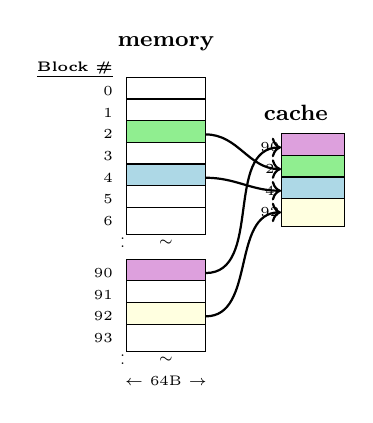
\begin{tikzpicture}[scale=0.55]
  % Define colors
  \definecolor{lightblue}{RGB}{173,216,230}
  \definecolor{lightgreen}{RGB}{144,238,144}
  \definecolor{lightyellow}{RGB}{255,255,224}
  \definecolor{lightpurple}{RGB}{221,160,221}
  
  % Memory column title
  \node[anchor=south, font=\footnotesize\bfseries] at (1.2, 4.1) {memory};
  \node[anchor=east, font=\tiny\bfseries] at (0.2, 3.9) {\underline{Block \#}};
  
  % Memory blocks with numbers
  \node[anchor=east, font=\tiny] at (0.2, 3.4) {0};
  \node[rectangle, draw, minimum width=1.0cm, minimum height=0.35cm, fill=white] (mem0) at (1.2, 3.4) {};
  
  \node[anchor=east, font=\tiny] at (0.2, 2.9) {1};
  \node[rectangle, draw, minimum width=1.0cm, minimum height=0.35cm, fill=white] (mem1) at (1.2, 2.9) {};
  
  \node[anchor=east, font=\tiny] at (0.2, 2.4) {2};
  \node[rectangle, draw, minimum width=1.0cm, minimum height=0.35cm, fill=lightgreen] (mem2) at (1.2, 2.4) {};
  
  \node[anchor=east, font=\tiny] at (0.2, 1.9) {3};
  \node[rectangle, draw, minimum width=1.0cm, minimum height=0.35cm, fill=white] (mem3) at (1.2, 1.9) {};
  
  \node[anchor=east, font=\tiny] at (0.2, 1.4) {4};
  \node[rectangle, draw, minimum width=1.0cm, minimum height=0.35cm, fill=lightblue] (mem4) at (1.2, 1.4) {};
  
  \node[anchor=east, font=\tiny] at (0.2, 0.9) {5};
  \node[rectangle, draw, minimum width=1.0cm, minimum height=0.35cm, fill=white] (mem5) at (1.2, 0.9) {};
  
  \node[anchor=east, font=\tiny] at (0.2, 0.4) {6};
  \node[rectangle, draw, minimum width=1.0cm, minimum height=0.35cm, fill=white] (mem6) at (1.2, 0.4) {};
  
  % Dots
  \node[font=\tiny] at (0.2, 0.0) {.};
  \node[font=\tiny] at (0.2, -0.2) {.};
  \node[font=\tiny] at (1.2, -0.1) {$\sim$};
  
  % Bottom memory blocks
  \node[anchor=east, font=\tiny] at (0.2, -0.8) {90};
  \node[rectangle, draw, minimum width=1.0cm, minimum height=0.35cm, fill=lightpurple] (mem90) at (1.2, -0.8) {};
  
  \node[anchor=east, font=\tiny] at (0.2, -1.3) {91};
  \node[rectangle, draw, minimum width=1.0cm, minimum height=0.35cm, fill=white] (mem91) at (1.2, -1.3) {};
  
  \node[anchor=east, font=\tiny] at (0.2, -1.8) {92};
  \node[rectangle, draw, minimum width=1.0cm, minimum height=0.35cm, fill=lightyellow] (mem92) at (1.2, -1.8) {};
  
  \node[anchor=east, font=\tiny] at (0.2, -2.3) {93};
  \node[rectangle, draw, minimum width=1.0cm, minimum height=0.35cm, fill=white] (mem93) at (1.2, -2.3) {};
  
  % More dots
  \node[font=\tiny] at (0.2, -2.7) {.};
  \node[font=\tiny] at (0.2, -2.9) {.};
  \node[font=\tiny] at (1.2, -2.8) {$\sim$};
  
  % 64B width indicator
  \node[anchor=center, font=\tiny] at (1.2, -3.3) {$\leftarrow$ 64B $\rightarrow$};
  
  % Cache column
  \node[anchor=south, font=\footnotesize\bfseries] at (4.2, 2.5) {cache};
  
  % Cache lines with block numbers
  \node[font=\tiny] at (3.6, 2.1) {90};
  \node[rectangle, draw, minimum width=0.8cm, minimum height=0.35cm, fill=lightpurple] (cache90) at (4.6, 2.1) {};
  
  \node[font=\tiny] at (3.6, 1.6) {2};
  \node[rectangle, draw, minimum width=0.8cm, minimum height=0.35cm, fill=lightgreen] (cache2) at (4.6, 1.6) {};
  
  \node[font=\tiny] at (3.6, 1.1) {4};
  \node[rectangle, draw, minimum width=0.8cm, minimum height=0.35cm, fill=lightblue] (cache4) at (4.6, 1.1) {};
  
  \node[font=\tiny] at (3.6, 0.6) {92};
  \node[rectangle, draw, minimum width=0.8cm, minimum height=0.35cm, fill=lightyellow] (cache92) at (4.6, 0.6) {};
  
  % Arrows from memory to cache
  \draw[->, thick] (mem90.east) to[out=0, in=180] (cache90.west);
  \draw[->, thick] (mem2.east) to[out=0, in=180] (cache2.west);
  \draw[->, thick] (mem4.east) to[out=0, in=180] (cache4.west);
  \draw[->, thick] (mem92.east) to[out=0, in=180] (cache92.west);
  
\end{tikzpicture}
\end{column}
\end{columns}
\end{frame}

\begin{frame}{Fully Associative (FA) Cache}
\begin{itemize}
  \item Any block can map to any line; tags of all lines are compared in parallel.
  \item Pros: lowest conflict misses. Cons: many comparators (area/power).
  \item On a tag match, return data using the offset.
\end{itemize}
\end{frame}

\begin{frame}{Valid Bit}
\begin{itemize}
  \item Cache starts empty; each line needs a \textbf{valid} bit.
  \item Valid set on fill; lines may be invalidated later.
\end{itemize}
\end{frame}

\begin{frame}{Direct-Mapped (DM) Cache}
\begin{itemize}
  \item Block number $\rightarrow$ \textbf{set} (index) + \textbf{tag}.
  \item Each block maps to exactly \emph{one} line: single comparator.
  \item Pros: simple, low power, fast. Cons: more \textbf{conflict} misses.
\end{itemize}
\end{frame}

\begin{frame}{2-Way Set Associative (2W SA)}
\begin{itemize}
  \item Each set holds 2 lines (ways); a block can reside in either way of its set.
  \item Requires two tag comparisons + way mux; fewer conflict misses than DM.
  \item Cache size $=\#\text{ways}\times\#\text{sets}\times\text{block size}$.
\end{itemize}
\end{frame}

\begin{frame}{2-Way Set Associative Cache -- Example}
% Define colors for the whole frame
\definecolor{tagcolor}{RGB}{100, 149, 237}    % Cornflower blue
\definecolor{setcolor}{RGB}{255, 140, 0}       % Dark orange
\definecolor{offsetcolor}{RGB}{220, 20, 60}    % Crimson
\definecolor{datacolor}{RGB}{240, 240, 240}    % Light gray

\begin{columns}[T]
\begin{column}{0.52\textwidth}
\centering
\begin{tikzpicture}[scale=0.95]
  
  % Address Fields section
  \node[anchor=west, font=\footnotesize\bfseries] at (0, 3.0) {Address Fields};
  
  % Bit numbers
  \node[font=\tiny] at (0.3, 2.6) {31};
  \node[font=\tiny] at (2.1, 2.6) {13};
  \node[font=\tiny] at (2.4, 2.6) {12};
  \node[font=\tiny] at (3.45, 2.6) {5};
  \node[font=\tiny] at (3.75, 2.6) {4};
  \node[font=\tiny] at (4.4, 2.6) {0};
  
  % Address fields boxes with colors
  \draw[thick, fill=tagcolor!20] (0.5, 2.1) rectangle (2.2, 2.4);
  \draw[thick, fill=setcolor!20] (2.2, 2.1) rectangle (3.6, 2.4);
  \draw[thick, fill=offsetcolor!20] (3.6, 2.1) rectangle (4.4, 2.4);
  
  \node[font=\tiny] at (1.35, 2.25) {\textcolor{tagcolor}{\textbf{Tag}}};
  \node[font=\tiny] at (2.9, 2.25) {\textcolor{setcolor}{\textbf{Set}}};
  \node[font=\tiny] at (4.0, 2.25) {\textcolor{offsetcolor}{\textbf{Offset}}};
  
  % Tag arrow
  \draw[->, thick, tagcolor, shorten >=0pt] (1.35, 2.1) -- (1.35, 1.6) -- (3.65, 1.6) -- (3.65, 0.9);

  % Improved arrows - Set arrow comes from left
  \draw[->, thick, setcolor, shorten >=0pt] (2.9, 2.1) -- (2.9, 1.8) -- (-0.3, 1.8) -- (-0.3, 0.1) -- (0.0, 0.1);
%  \draw[->, thick, setcolor, shorten >=0pt] (-0.3, 0.1) -- (2.7, 0.1);
  
  % Cache structure - Way #0
  \node[font=\footnotesize\bfseries] at (1.4, -1.9) {Way 0};
  
  % Tag Array Way 0 with taller rows
  \draw[thick] (0.5, 0.9) rectangle (1.4, -1.1);
  \foreach \y in {0.65, 0.35, 0.05, -0.25, -0.55, -0.85}
    \draw (0.5, \y) -- (1.4, \y);
  % Fill with tag color
  \fill[tagcolor!15] (0.5, 0.9) rectangle (1.4, -1.1);
  % Add some specific entries
  \node[font=\tiny] at (0.95, 0.5) {091A2};
  \node[font=\tiny] at (0.95, 0.2) {...};
  \node[font=\tiny] at (0.95, -0.1) {...};
  \node[font=\tiny] at (0.95, -0.4) {...};
  \node[font=\tiny] at (0.95, -0.7) {...};
  \node[font=\tiny] at (0.95, -1.0) {...};
  
  % Data Array Way 0 with taller rows
  \draw[thick] (1.4, 0.9) rectangle (2.5, -1.1);
  \foreach \y in {0.65, 0.35, 0.05, -0.25, -0.55, -0.85}
    \draw (1.4, \y) -- (2.5, \y);
  \fill[datacolor] (1.4, 0.9) rectangle (2.5, -1.1);
  
  % Labels for Way 0
  \node[font=\tiny, rotate=90] at (0.95, 1.2) {\textcolor{tagcolor}{\textbf{Tag}}};
  \node[font=\tiny, rotate=90] at (1.95, 1.2) {\textbf{Data}};
  
  \node[font=\tiny] at (0.95, -1.35) {\textcolor{tagcolor}{Tag}};
  \node[font=\tiny] at (0.95, -1.5) {\textcolor{tagcolor}{Array}};
  \node[font=\tiny] at (1.95, -1.35) {Data};
  \node[font=\tiny] at (1.95, -1.5) {Array};
  
  % Cache structure - Way #1
  \node[font=\footnotesize\bfseries] at (4.0, -1.9) {Way 1};
  
  % Tag Array Way 1 with taller rows
  \draw[thick] (3.2, 0.9) rectangle (4.1, -1.1);
  \foreach \y in {0.65, 0.35, 0.05, -0.25, -0.55, -0.85}
    \draw (3.2, \y) -- (4.1, \y);
  % Fill with tag color
  \fill[tagcolor!15] (3.2, 0.9) rectangle (4.1, -1.1);
  
  % Data Array Way 1 with taller rows
  \draw[thick] (4.1, 0.9) rectangle (5.2, -1.1);
  \foreach \y in {0.65, 0.35, 0.05, -0.25, -0.55, -0.85}
    \draw (4.1, \y) -- (5.2, \y);
  \fill[datacolor] (4.1, 0.9) rectangle (5.2, -1.1);
  
  % Labels for Way 1
  \node[font=\tiny, rotate=90] at (3.65, 1.2) {\textcolor{tagcolor}{\textbf{Tag}}};
  \node[font=\tiny, rotate=90] at (4.65, 1.2) {\textbf{Data}};
  
  \node[font=\tiny] at (3.65, -1.35) {\textcolor{tagcolor}{Tag}};
  \node[font=\tiny] at (3.65, -1.5) {\textcolor{tagcolor}{Array}};
  \node[font=\tiny] at (4.65, -1.35) {Data};
  \node[font=\tiny] at (4.65, -1.5) {Array};
  
  
\end{tikzpicture}
\end{column}

\begin{column}{0.48\textwidth}
\footnotesize
\begin{tabular}{ll}
\textbf{Line Size:} & $32$ bytes $= 2^5$ bytes\\
\textbf{Cache Size:} & $16$ KB $= 2^{14}$ bytes\\
\textbf{\# Lines:} & $\frac{\text{cache size}}{\text{line size}} = \frac{2^{14}}{2^5} = 512$ lines\\
\textbf{\# Ways:} & $2$\\
\textbf{\# Sets:} & $\frac{\text{\#lines}}{\text{\#ways}} = 256$ sets
\end{tabular}

\vspace{0.2cm}
\begin{tabular}{ll}
\textcolor{offsetcolor}{\textbf{Offset bits:}} & $\log_2(\text{line size}) = 5$ bits\\
\textcolor{setcolor}{\textbf{Set bits:}} & $\log_2(\text{\#sets}) = 8$ bits\\
\textcolor{tagcolor}{\textbf{Tag bits:}} & $32 - (5+8) = 19$ bits\\
\end{tabular}

\vspace{0.3cm}
\textbf{Example:} Address \texttt{0x12345678}\\[2pt]
{\texttt{%
\textcolor{tagcolor}{0001 0010 0011 0100 010}%
\textcolor{setcolor}{1 0110 011}%
\textcolor{offsetcolor}{1 1000}}}\\[4pt]

\footnotesize
\begin{tabular}{ll}
\textcolor{offsetcolor}{\textbf{Offset:}} & \texttt{11000} $= \mathtt{0x18}$\\
\textcolor{setcolor}{\textbf{Set:}} & \texttt{10110011} $= \mathtt{0xB3}$\\
\textcolor{tagcolor}{\textbf{Tag:}} & \texttt{0001001000110100010}\\
                     & $= \mathtt{0x091A2}$\\
\end{tabular}
\end{column}
\end{columns}
\end{frame}


\begin{frame}{2-Way Set Associative vs. Direct Map Cache}

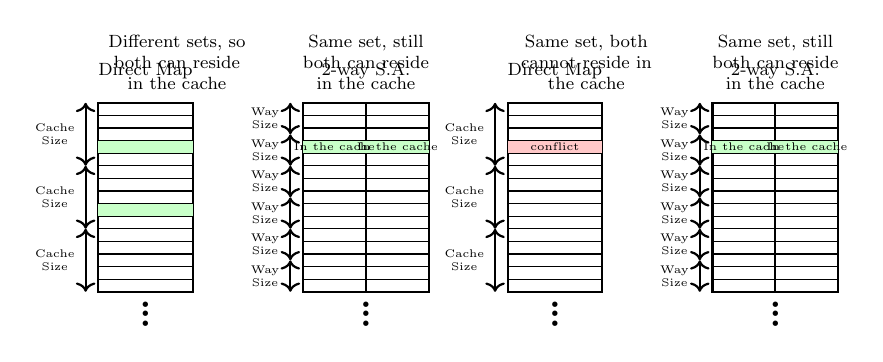
\begin{tikzpicture}[scale=0.8, transform shape]
  % Define colors
  \definecolor{lightgreen}{RGB}{200,255,200}
  \definecolor{lightred}{RGB}{255,200,200}
  
  % First scenario - Different sets
  \begin{scope}[shift={(0,0)}]
    \node[anchor=north, align=center, font=\footnotesize] at (1.25, 4.2) {Different sets, so\\both can reside\\in the cache};
    
    % Direct Map
    \node[font=\footnotesize] at (0.75, 3.5) {Direct Map};
    \draw[thick] (0, 0) rectangle (1.5, 3);
    
    % Draw cache lines with some colored
    \foreach \y in {0, 0.2, ..., 2.8} {
      \draw (0, \y) -- (1.5, \y);
    }
    \fill[lightgreen] (0, 1.2) rectangle (1.5, 1.4);
    \fill[lightgreen] (0, 2.2) rectangle (1.5, 2.4);
    
    % Cache Size labels
    \draw[<->, thick] (-0.2, 0) -- (-0.2, 1);
    \node[anchor=east, font=\tiny, align=center] at (-0.25, 0.5) {Cache\\Size};
    
    \draw[<->, thick] (-0.2, 1) -- (-0.2, 2);
    \node[anchor=east, font=\tiny, align=center] at (-0.25, 1.5) {Cache\\Size};
    
    \draw[<->, thick] (-0.2, 2) -- (-0.2, 3);
    \node[anchor=east, font=\tiny, align=center] at (-0.25, 2.5) {Cache\\Size};
    
    % Dots below
    \foreach \y in {-0.2, -0.35, -0.5} {
      \node at (0.75, \y) {\tiny$\bullet$};
    }
  \end{scope}
  
  % Second scenario - Same set, still both can reside (2-way)
  \begin{scope}[shift={(3,0)}]
    \node[anchor=north, align=center, font=\footnotesize] at (1.25, 4.2) {Same set, still\\both can reside\\in the cache};
    
    % 2-way S.A.
    \node[font=\footnotesize] at (1.25, 3.5) {2-way S.A.};
    \draw[thick] (0.25, 0) rectangle (2.25, 3);
    \draw[thick] (1.25, 0) -- (1.25, 3); % Vertical divider
    
    % Draw cache lines
    \foreach \y in {0, 0.2, ..., 2.8} {
      \draw (0.25, \y) -- (2.25, \y);
    }
    \fill[lightgreen] (0.25, 2.2) rectangle (1.25, 2.4);
    \fill[lightgreen] (1.25, 2.2) rectangle (2.25, 2.4);
    
    % Way Size labels
    \draw[<->, thick] (0.05, 0) -- (0.05, 0.5);
    \node[anchor=east, font=\tiny, align=center] at (0, 0.25) {Way\\Size};
    
    \draw[<->, thick] (0.05, 0.5) -- (0.05, 1);
    \node[anchor=east, font=\tiny, align=center] at (0, 0.75) {Way\\Size};
    
    \draw[<->, thick] (0.05, 1) -- (0.05, 1.5);
    \node[anchor=east, font=\tiny, align=center] at (0, 1.25) {Way\\Size};
    
    \draw[<->, thick] (0.05, 1.5) -- (0.05, 2);
    \node[anchor=east, font=\tiny, align=center] at (0, 1.75) {Way\\Size};
    
    \draw[<->, thick] (0.05, 2) -- (0.05, 2.5);
    \node[anchor=east, font=\tiny, align=center] at (0, 2.25) {Way\\Size};
    
    \draw[<->, thick] (0.05, 2.5) -- (0.05, 3);
    \node[anchor=east, font=\tiny, align=center] at (0, 2.75) {Way\\Size};
    
    % In the cache labels
    \node[font=\tiny] at (0.75, 2.3) {In the cache};
    \node[font=\tiny] at (1.75, 2.3) {In the cache};
    
    % Dots below
    \foreach \y in {-0.2, -0.35, -0.5} {
      \node at (1.25, \y) {\tiny$\bullet$};
    }
  \end{scope}
  
  % Third scenario - Same set, cannot reside (Direct Map)
  \begin{scope}[shift={(6.5,0)}]
    \node[anchor=north, align=center, font=\footnotesize] at (1.25, 4.2) {Same set, both\\cannot reside in\\the cache};
    
    % Direct Map
    \node[font=\footnotesize] at (0.75, 3.5) {Direct Map};
    \draw[thick] (0, 0) rectangle (1.5, 3);
    
    % Draw cache lines
    \foreach \y in {0, 0.2, ..., 2.8} {
      \draw (0, \y) -- (1.5, \y);
    }
    % Red overlapping blocks
    \fill[lightred] (0, 2.2) rectangle (1.5, 2.4);
    
    % Cache Size labels
    \draw[<->, thick] (-0.2, 0) -- (-0.2, 1);
    \node[anchor=east, font=\tiny, align=center] at (-0.25, 0.5) {Cache\\Size};
    
    \draw[<->, thick] (-0.2, 1) -- (-0.2, 2);
    \node[anchor=east, font=\tiny, align=center] at (-0.25, 1.5) {Cache\\Size};
    
    \draw[<->, thick] (-0.2, 2) -- (-0.2, 3);
    \node[anchor=east, font=\tiny, align=center] at (-0.25, 2.5) {Cache\\Size};
    
    % Conflict label
    \node[font=\tiny, align=center] at (0.75, 2.3) {conflict};
    
    % Dots below
    \foreach \y in {-0.2, -0.35, -0.5} {
      \node at (0.75, \y) {\tiny$\bullet$};
    }
  \end{scope}
  
  % Fourth scenario - Same set, still both can reside (2-way)
  \begin{scope}[shift={(9.5,0)}]
    \node[anchor=north, align=center, font=\footnotesize] at (1.25, 4.2) {Same set, still\\both can reside\\in the cache};
    
    % 2-way S.A.
    \node[font=\footnotesize] at (1.25, 3.5) {2-way S.A.};
    \draw[thick] (0.25, 0) rectangle (2.25, 3);
    \draw[thick] (1.25, 0) -- (1.25, 3); % Vertical divider
    
    % Draw cache lines
    \foreach \y in {0, 0.2, ..., 2.8} {
      \draw (0.25, \y) -- (2.25, \y);
    }
    \fill[lightgreen] (0.25, 2.2) rectangle (1.25, 2.4);
    \fill[lightgreen] (1.25, 2.2) rectangle (2.25, 2.4);
    
    % Way Size labels
    \draw[<->, thick] (0.05, 0) -- (0.05, 0.5);
    \node[anchor=east, font=\tiny, align=center] at (0, 0.25) {Way\\Size};
    
    \draw[<->, thick] (0.05, 0.5) -- (0.05, 1);
    \node[anchor=east, font=\tiny, align=center] at (0, 0.75) {Way\\Size};
    
    \draw[<->, thick] (0.05, 1) -- (0.05, 1.5);
    \node[anchor=east, font=\tiny, align=center] at (0, 1.25) {Way\\Size};
    
    \draw[<->, thick] (0.05, 1.5) -- (0.05, 2);
    \node[anchor=east, font=\tiny, align=center] at (0, 1.75) {Way\\Size};
    
    \draw[<->, thick] (0.05, 2) -- (0.05, 2.5);
    \node[anchor=east, font=\tiny, align=center] at (0, 2.25) {Way\\Size};
    
    \draw[<->, thick] (0.05, 2.5) -- (0.05, 3);
    \node[anchor=east, font=\tiny, align=center] at (0, 2.75) {Way\\Size};
    
    % In the cache labels
    \node[font=\tiny] at (0.75, 2.3) {In the cache};
    \node[font=\tiny] at (1.75, 2.3) {In the cache};
    
    % Dots below
    \foreach \y in {-0.2, -0.35, -0.5} {
      \node at (1.25, \y) {\tiny$\bullet$};
    }
  \end{scope}
  
\end{tikzpicture}

\end{frame}



\begin{frame}[fragile]{LRU Implementation}
\begin{columns}[T]
\begin{column}{0.70\textwidth}
\begin{itemize}
  \item \textcolor{blue}{\textbf{2 ways}}
  \begin{itemize}
    \item 1 bit per set to mark the most recently accessed way in the set
    \item Evict the way which is not pointed to by the bit
  \end{itemize}
  
  \item \textcolor{blue}{\textbf{k-way set associative LRU}}
  \begin{itemize}
    \item For each set maintain the way access order \\
    $\Rightarrow$ per set: log$_2$k bit counter per way
    \begin{itemize}
      \item 4 ways: 4$\times$2 bits per set; 8 ways: 8$\times$3 bits per set
      \item Many bits $\Rightarrow$ complicated update scheme
    \end{itemize}
    \item When way $i$ is accessed:
    \item When replacement is needed: evict the way with counter = 0
  \end{itemize}
  
  \begin{block}{Pseudo-code (on access of way $i$)}
  \begin{lstlisting}[basicstyle=\ttfamily\small]
X = Counter[i]
Counter[i] = k-1          // way i becomes MRU
for j in [0..k-1]:
  if j != i and Counter[j] > X: Counter[j]--
  \end{lstlisting}
  \end{block}
\end{itemize}
\end{column}

\begin{column}{0.30\textwidth}
\small
\raggedright
\textbf{Initial State}\\
\vspace{0.1cm}
\begin{tabular}{|c|c|c|c|c|}
\hline
Way & 0 & 1 & 2 & 3 \\
\hline
Count & 0 & 1 & 2 & 3 \\
\hline
\end{tabular}

\vspace{0.4cm}
\textbf{$\Rightarrow$ Access way 2}\\
\vspace{0.1cm}
\begin{tabular}{|c|c|c|c|c|}
\hline
Way & 0 & 1 & 2 & 3 \\
\hline
Count & 0 & 1 & \textcolor{red}{\textbf{3}} & 2 \\
\hline
\end{tabular}

\vspace{0.4cm}
\textbf{$\Rightarrow$ Access way 0}\\
\vspace{0.1cm}
\begin{tabular}{|c|c|c|c|c|}
\hline
Way & 0 & 1 & 2 & 3 \\
\hline
Count & \textcolor{red}{\textbf{3}} & 0 & 2 & 1 \\
\hline
\end{tabular}
\end{column}
\end{columns}
\end{frame}

\begin{frame}{Pseudo LRU (PLRU)}
\begin{columns}
\begin{column}{0.75\textwidth}
\begin{itemize}
  \item \textbf{PLRU records partial order using tree structure}
  \begin{itemize}
    \item Ways at leaves; PLRU bits at internal nodes
    \item For $n$ leaves: $n-1$ internal nodes (PLRU bits)
  \end{itemize}
  
  \vspace{0.2cm}
  
  \item \textbf{Example: 4-way cache, 3 bits per set}
  \begin{itemize}
    \item Bit$_0$: order between \{0,1\} and \{2,3\}
    \item Bit$_1$: order between ways 0 and 1
    \item Bit$_2$: order between ways 2 and 3
  \end{itemize}
  
  \vspace{0.2cm}
  
  \item \textbf{Update on access: point to accessed way}
  \begin{itemize}
    \item 0=left, 1=right
    \item After accessing 0→3→2→1:
    \begin{itemize}
      \item bit$_0$=0 → pair with way 1 (MRU)
      \item bit$_1$=1 → way 1 (MRU)
      \item bit$_2$=0 → way 2 over way 3
    \end{itemize}
  \end{itemize}
  
  \vspace{0.2cm}
  
  \item \textbf{Victim selection: follow opposite direction}
  \begin{itemize}
    \item 0=right, 1=left
    \item \textcolor{red}{May not select true LRU}
  \end{itemize}
\end{itemize}
\end{column}

\begin{column}{0.25\textwidth}
\centering
\vspace{-0.5cm}

\textbf{Initial Tree:}

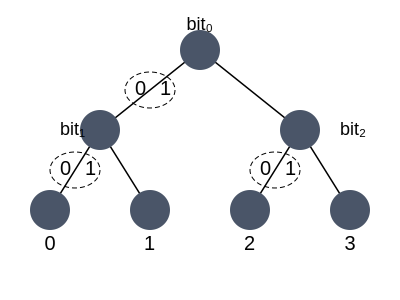
\includegraphics[width=\textwidth]{svg/cache_plru_initial.pdf}

\vspace{0.3cm}

\textbf{After accessing 0→3→2→1:}

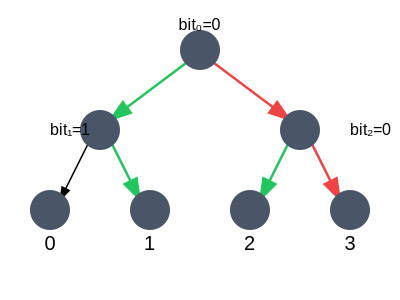
\includegraphics[width=\textwidth]{svg/cache_plru_after_access.pdf}

\vspace{0.2cm}
\small
\textcolor{red}{Victim: Way 3} \\
\textcolor{blue}{MRU: Way 1}
\end{column}
\end{columns}
\end{frame}

\begin{frame}{Cache Line Size Trade-offs}
\begin{itemize}
  \item Larger lines exploit spatial locality but may fetch unused data $\rightarrow$ more evictions
  \item Larger lines increase \textbf{miss penalty}; ``critical word first'' helps
  \item $t_{\text{avg}} = t_{hit}\cdot(1-\text{MR}) + t_{miss}\cdot \text{MR}$
\end{itemize}
\end{frame}


\begin{frame}{Effect of Cache on Performance}

\begin{itemize}
  \item \textbf{MPI — misses per instruction}
  \begin{itemize}
    \item MPI = $\frac{\text{\#cache misses}}{\text{\#instructions}} = \frac{\text{\#cache misses}}{\text{\#mem accesses}} \times \frac{\text{\#mem accesses}}{\text{\#instructions}}$
    \item More correlative to performance than cache miss rate
    \begin{itemize}
      \item Takes into account also frequency of memory accesses
    \end{itemize}
  \end{itemize}
  
  \vspace{0.4cm}
  
  \item[\textcolor{blue}{$\diamond$}] \textbf{Memory stall cycles}
  \begin{itemize}
    \item[] = \#memory accesses $\times$ miss rate $\times$ miss penalty
    \item[] = IC $\times$ MPI $\times$ miss penalty
  \end{itemize}
  
  \vspace{0.4cm}
  
  \item[\textcolor{blue}{$\diamond$}] \textbf{CPU time}
  \begin{itemize}
    \item[] = (CPU execution cycles + Memory stall cycles) $\times$ cycle time
    \item[] = IC $\times$ (CPI$_{\text{execution}}$ + MPI $\times$ Miss penalty) $\times$ cycle time
  \end{itemize}
\end{itemize}

\end{frame}

\begin{frame}{Classifying Misses: The 3Cs}
\begin{itemize}
  \item \textbf{Compulsory}: first reference to a block $\Rightarrow$ use prefetch to mitigate
  \item \textbf{Capacity}: working set $>$ cache size $\Rightarrow$ increase size / use stream buffers
  \item \textbf{Conflict}: set mapping causes evictions $\Rightarrow$ use higher associativity / victim cache
\end{itemize}
\end{frame}


\begin{frame}{Fill Buffer Architecture}
\begin{center}
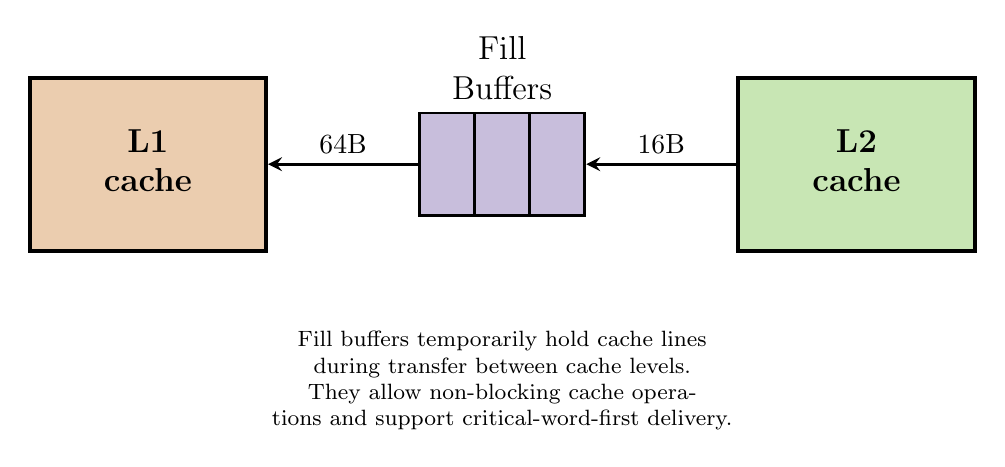
\begin{tikzpicture}[
    cache/.style={rectangle, draw=black, line width=1.5pt, minimum width=3cm, minimum height=2.2cm, font=\large},
    buffer/.style={rectangle, draw=black, line width=1pt, minimum width=0.7cm, minimum height=1.3cm, fill=buffercolor},
    arrow/.style={->, >=stealth, line width=1.2pt, black},
    label/.style={font=\normalsize, black}
]

% Define colors that match your presentation style
\definecolor{l1color}{RGB}{235, 205, 175}
\definecolor{l2color}{RGB}{200, 230, 180}
\definecolor{buffercolor}{RGB}{200, 190, 220}

% L1 Cache
\node[cache, fill=l1color] (l1) at (0,0) {
    \begin{tabular}{c}
        \textbf{L1}\\
        \textbf{cache}
    \end{tabular}
};

% Fill Buffers label
\node[above, font=\large] at (4.5,1.2) {Fill};
\node[above, font=\large] at (4.5,0.7) {Buffers};

% Individual buffer blocks
\node[buffer] (buf1) at (3.8,0) {};
\node[buffer] (buf2) at (4.5,0) {};
\node[buffer] (buf3) at (5.2,0) {};

% L2 Cache
\node[cache, fill=l2color] (l2) at (9,0) {
    \begin{tabular}{c}
        \textbf{L2}\\
        \textbf{cache}
    \end{tabular}
};

% Arrows with labels (corrected direction: L2 -> buffers -> L1)
\draw[arrow] (l2.west) -- node[above, label] {16B} (buf3.east);
\draw[arrow] (buf1.west) -- node[above, label] {64B} (l1.east);

% Optional: Add some detail text below
\node[below, font=\footnotesize, text width=10cm, align=center] at (4.5,-2) {
    Fill buffers temporarily hold cache lines during transfer between cache levels.\\
    They allow non-blocking cache operations and support critical-word-first delivery.
};

\end{tikzpicture}
\end{center}
\end{frame}

\begin{frame}{Cache Line Fill and Fill Buffers}
\begin{columns}[T]
\begin{column}{0.7\textwidth}
\begin{itemize}
  \item Before inserting a new line into cache
  \begin{itemize}
    \item Put new line in a fill buffer
  \end{itemize}
  
  \item Bus width considerations
  \begin{itemize}
    \item L2 to L1 bus may be narrower than cache line size
    \item E.g., 16B bus width, 64B cache line $\Rightarrow$ 4 bus cycles
    \item Fetch critical chunk (containing missed address) first
    \item Fill buffer accumulates full line, then writes to cache
    \item Search fill buffers in parallel with cache for data forwarding
  \end{itemize}
  
  \item Streaming loads optimization
  \begin{itemize}
    \item SW/compiler hints for single-use data
    \item E.g., scanning large arrays once
    \item Line unlikely to be reused $\Rightarrow$ avoid cache pollution
    \item Serve data directly from fill buffer without cache insertion
  \end{itemize}
\end{itemize}
\end{column}

\begin{column}{0.3\textwidth}
\begin{center}
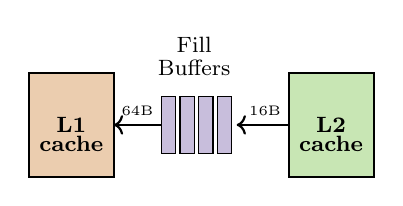
\begin{tikzpicture}[scale=0.6]
  % Define colors
  \definecolor{l1color}{RGB}{235, 205, 175}
  \definecolor{l2color}{RGB}{200, 230, 180}
  \definecolor{buffercolor}{RGB}{200, 190, 220}
  
  % L1 Cache
  \draw[thick, fill=l1color] (0,0) rectangle (1.8,2.2);
  \node[font=\footnotesize\bfseries] at (0.9,1.1) {L1};
  \node[font=\footnotesize\bfseries] at (0.9,0.7) {cache};
  
  % Fill Buffers
  \node[font=\footnotesize] at (3.5,2.8) {Fill};
  \node[font=\footnotesize] at (3.5,2.3) {Buffers};
  \foreach \i in {0,1,2,3} {
    \draw[fill=buffercolor] ({2.8+\i*0.4},0.5) rectangle ({3.1+\i*0.4},1.7);
  }
  
  % L2 Cache
  \draw[thick, fill=l2color] (5.5,0) rectangle (7.3,2.2);
  \node[font=\footnotesize\bfseries] at (6.4,1.1) {L2};
  \node[font=\footnotesize\bfseries] at (6.4,0.7) {cache};
  
  % Arrows with correct direction (L2 -> buffers -> L1)
  \draw[->, thick] (5.5,1.1) -- (4.4,1.1);
  \draw[->, thick] (2.8,1.1) -- (1.8,1.1);
  
  % Labels
  \node[font=\tiny] at (5.0,1.4) {16B};
  \node[font=\tiny] at (2.3,1.4) {64B};
\end{tikzpicture}
\end{center}
\end{column}
\end{columns}
\end{frame}

% Alternative version with more detail
\begin{frame}{Fill Buffer Operation}
\begin{columns}[T]
\begin{column}{0.6\textwidth}
\begin{itemize}
  \item \textbf{Fill buffers bridge cache levels}
  \begin{itemize}
    \item Hold incoming cache lines from L2/memory
    \item Allow critical word first delivery
    \item Enable hit-under-miss operation
  \end{itemize}
  
  \vspace{0.3cm}
  
  \item \textbf{Key characteristics:}
  \begin{itemize}
    \item Typically 4-8 entries
    \item Each holds one cache line
    \item Searched in parallel with L1
    \item Can forward data before line fills complete
  \end{itemize}
\end{itemize}
\end{column}

\begin{column}{0.4\textwidth}
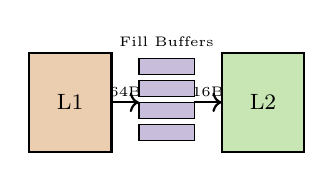
\begin{tikzpicture}[scale=0.7]
% Define colors
\definecolor{l1color}{RGB}{235, 205, 175}
\definecolor{l2color}{RGB}{200, 230, 180}
\definecolor{buffercolor}{RGB}{200, 190, 220}

% L1 Cache (smaller)
\draw[thick, fill=l1color] (0,0) rectangle (1.5,1.8);
\node[font=\footnotesize] at (0.75,0.9) {L1};

% Fill Buffers
\node[font=\tiny] at (2.5,2) {Fill Buffers};
\foreach \y in {0.2, 0.6, 1.0, 1.4} {
    \draw[fill=buffercolor] (2,\y) rectangle (3,{\y+0.3});
}

% L2 Cache (smaller)
\draw[thick, fill=l2color] (3.5,0) rectangle (5,1.8);
\node[font=\footnotesize] at (4.25,0.9) {L2};

% Arrows
\draw[->, thick] (1.5,0.9) -- (2,0.9);
\draw[->, thick] (3,0.9) -- (3.5,0.9);

% Labels
\node[font=\tiny] at (1.75,1.1) {64B};
\node[font=\tiny] at (3.25,1.1) {16B};
\end{tikzpicture}
\end{column}
\end{columns}
\end{frame}




\begin{frame}{Line Fill and Fill Buffers}
\begin{itemize}
  \item Missed block arrives in chunks; critical-chunk-first reduces latency
  \item Fill buffer accumulates the full line, then writes to cache; also searched on access
  \item ``Streaming'' loads may bypass L1 fill to avoid pollution
\end{itemize}
\end{frame}

\begin{frame}{Victim Cache}
\begin{itemize}
  \item Small FA cache that holds lines evicted from L1.
  \item Checked in parallel with L1; on hit, swap victim back to L1.
  \item Reduces conflict pressure, especially for direct-mapped L1.
\end{itemize}
\end{frame}

\begin{frame}{Memory Updates on Writes}
\begin{columns}[T]
\column{0.5\textwidth}
\textbf{Write-back}
\begin{itemize}
  \item Write hits update only cache; line marked \emph{dirty}.
  \item Evict: write entire line to next level.
\end{itemize}
\column{0.5\textwidth}
\textbf{Write-through}
\begin{itemize}
  \item Write hits update cache \emph{and} next level.
  \item Needs a write buffer; evictions are clean.
\end{itemize}
\end{columns}
\end{frame}

\begin{frame}{Write Buffer \& Write Combining}
\begin{itemize}
  \item Buffer decouples CPU stores from DRAM writes.
  \item Combine multiple writes to same line into one buffer entry.
  \item On a miss, also consult write buffer for the most up-to-date bytes.
\end{itemize}
\end{frame}

\begin{frame}{Cache Write Miss}
\begin{itemize}
  \item \textbf{The processor is not waiting for data}
  \begin{itemize}
    \item[$\Rightarrow$] continues its work
  \end{itemize}
  
  \vspace{0.5cm}
  
  \item \textbf{Option 1: Write-allocate: fetch the write miss line into the cache}
  \begin{itemize}
    \item[\textcolor{green}{$\checkmark$}] Goes with \textit{write back} policy, assuming more writes are needed
    \item[\textcolor{green}{$\checkmark$}] Hoping that subsequent writes to the line hit the cache
  \end{itemize}
  
  \vspace{0.5cm}
  
  \item \textbf{Option 2: Write-no-allocate: do not fetch the write miss line into the cache}
  \begin{itemize}
    \item[\textcolor{green}{$\checkmark$}] Goes with \textit{write through} policy
    \item[\textcolor{green}{$\checkmark$}] Subsequent writes would update memory anyhow
  \end{itemize}
\end{itemize}
\end{frame}

\begin{frame}{Prefetching}
\begin{itemize}
  \item \textbf{Hardware Data Prefetching -- predict future data accesses}
  \begin{itemize}
    \item Next sequential / Streaming prefetcher
    \begin{itemize}
      \item Triggered by an ascending access to very recently loaded data
      \item Fetches the next line, assuming a streaming load
    \end{itemize}
    \item Stride prefetcher
    \begin{itemize}
      \item Tracks individual load instructions, detecting a regular stride
      \item Prefetch address = current address + stride
      \item Both forward and backward
    \end{itemize}
    \item General pattern prefetcher
    \begin{itemize}
      \item Identifies patterns of Load address distances
    \end{itemize}
  \end{itemize}
  
  \item \textbf{Data has to be prefetched before it is needed}
  \begin{itemize}
    \item The prefetcher aggressiveness has to be tuned
    \item How fast and how far ahead to issue the prefetch request, such that data arrives on time, before it is needed
  \end{itemize}
\end{itemize}
\end{frame}

\begin{frame}{Prefetching (cont.)}
\begin{itemize}
  \item \textbf{Prefetching relies on extra memory bandwidth}
  \begin{itemize}
    \item Too aggressive / inaccurate prefetching slows down demand fetches and pollutes the cache
    \begin{itemize}
      \item Hurts performance
    \end{itemize}
  \end{itemize}
  
  \item \textbf{Software Prefetching}
  \begin{itemize}
    \item Special prefetching instructions that cannot cause faults
  \end{itemize}
  
  \item \textbf{Instruction Prefetching}
  \begin{itemize}
    \item On a cache miss, prefetch sequential cache lines into stream buffers
    \item Branch predictor directed prefetching
    \begin{itemize}
      \item Let branch predictor run ahead
    \end{itemize}
  \end{itemize}
\end{itemize}
\end{frame}

\begin{frame}{Code Optimizations for Locality}
\begin{itemize}
  \item \textbf{Merging arrays}: AoS vs SoA trade-offs; reduce conflicts, improve spatial locality.
  \item \textbf{Loop fusion}: combine loops with same traversal to increase reuse.
  \item \textbf{Loop interchange}: access arrays in memory order to exploit spatial locality.
\end{itemize}
\end{frame}



\begin{frame}[fragile]{Code Optimizations: Merging Arrays}
\begin{itemize}
  \item \textbf{Merge 2 arrays into a single array of compound elements}
\end{itemize}

\begin{columns}
\begin{column}{0.65\textwidth}
\begin{block}{Before: two sequential arrays}
\small
\begin{lstlisting}[basicstyle=\ttfamily\small, commentstyle=\color{red}]
int val[SIZE];
int key[SIZE];
\end{lstlisting}
\end{block}

\begin{block}{After: One array of structures}
\small
\begin{lstlisting}[basicstyle=\ttfamily\small, commentstyle=\color{green!60!black}]
struct merge {
    int val;
    int key;
} merged_array[SIZE];
\end{lstlisting}
\end{block}
\end{column}

\begin{column}{0.35\textwidth}
\begin{itemize}
  \item[$\diamond$] \textbf{Reduce conflicts between val and key}
  \item[$\diamond$] \textbf{Improves spatial locality}
\end{itemize}
\end{column}
\end{columns}
\end{frame}

\begin{frame}[fragile]{Code Optimizations: Loop Fusion}
\begin{itemize}
  \item \textbf{Merge loops with shared data access}
  \item Assume each element in \texttt{a} is 4 bytes, 32KB cache, 32 B/line
\end{itemize}

\begin{columns}
\begin{column}{0.55\textwidth}
\begin{block}{Before Fusion}
\small
\texttt{for (i = 0; i < 10000; i++)}\\
\texttt{~~a[i] = 1 / a[i];}\\
\texttt{for (i = 0; i < 10000; i++)}\\
\texttt{~~sum = sum + a[i];}
\end{block}

\vspace{0.2cm}
\begin{block}{After Fusion}
\small
\texttt{for (i = 0; i < 10000; i++) \{}\\
\texttt{~~a[i] = 1 / a[i];}\\
\texttt{~~sum = sum + a[i];}\\
\texttt{\}}
\end{block}
\end{column}

\begin{column}{0.45\textwidth}
%\textbf{Before Fusion:}
\begin{itemize}
  \item[\textcolor{green}{$\diamond$}] First loop: hit in 7/8 of iterations
  \item[\textcolor{green}{$\diamond$}] Second loop: $\text{array} > \text{cache}$ $\Rightarrow$ same hit rate as in 1\textsuperscript{st} loop
\end{itemize}

\vspace{1cm}
%\textbf{After Fusion:}
\begin{itemize}
  \item[\textcolor{green}{$\diamond$}] First line: hit in 7/8 of iterations
  \item[\textcolor{green}{$\diamond$}] Second line: hit in all
\end{itemize}

\vspace{0.2cm}
\footnotesize
\textit{Note: Only load accesses are considered for hit rate calculation}
\end{column}
\end{columns}
\end{frame}

\begin{frame}[fragile]{Code Optimizations: Loop Interchange}
\begin{itemize}
  \item \textbf{2-dimensional array in memory:}
\end{itemize}

\small
\texttt{x[0][0] x[0][1] ... x[0][99] x[1][0] x[1][1] ...}

\vspace{0.3cm}
\begin{block}{Original program: accesses are 100 bytes apart}
\small
\texttt{/* x[0][0] x[1][0] ... x[4999][0] x[0][1] x[1][1] ... */}\\
\texttt{for (j = 0; j < 100; j++)}\\
\texttt{~~for (i = 0; i < 5000; i++)}\\
\texttt{~~~~x[i][j] = 2 * x[i][j];}
\end{block}

\vspace{0.2cm}
\begin{block}{Reversing the loop order: accesses are adjacent}
\small
\texttt{/* Improved spatial locality */}\\
\begin{tikzpicture}[overlay, remember picture]
  \coordinate (top) at (7.5,0);
  \coordinate (bottom) at (7.5,-0.4);
  \draw[<->, thick, green!70!black, line width=1.5pt, bend right=60] 
    (top) to (bottom);
  \node[green!70!black, right, font=\scriptsize] at (8.0,-0.2) {swap};
\end{tikzpicture}
\texttt{for (i = 0; i < 5000; i++)}\\
\texttt{~~for (j = 0; j < 100; j++)}\\
\texttt{~~~~x[i][j] = 2 * x[i][j];}
\end{block}
\end{frame}

\begin{frame}{Improving Cache Performance (summary)}
\begin{itemize}
  \item \textbf{Reduce miss rate}: bigger caches/lines, higher associativity, victim cache, stream buffers, prefetching, compiler transforms
  \item \textbf{Reduce miss penalty}: early restart/critical word first, non-blocking caches, L2/L3
  \item \textbf{Reduce hit time}: smaller, on-chip, direct-mapped L1
\end{itemize}
\end{frame}

\begin{frame}{Split I-Cache / D-Cache}
\begin{itemize}
  \item Parallel fetch and data access in different pipeline stages
  \item Different characteristics: I$:$ read-only; D$:$ reads and writes; different prefetching
  \item Self-modifying code: snoop I-cache tags and invalidate on matching store
\end{itemize}
\end{frame}

\begin{frame}{Non-Blocking Caches}
\begin{itemize}
  \item \textbf{Hit Under Miss}
  \begin{itemize}
    \item Allow cache hits while one miss is in progress
    \item Another miss has to wait
    \item Relevant for an out-of-order execution CPU
  \end{itemize}
  \vspace{0.2cm}
  \item \textbf{Miss Under Miss, Hit Under Multiple Misses}
  \begin{itemize}
    \item Allow hits and misses when other misses in progress
    \item Memory system must allow multiple pending requests
    \item Manage a list of outstanding cache misses
    \begin{itemize}
      \item When miss is served and data gets back, update list
    \end{itemize}
  \end{itemize}
\end{itemize}
\end{frame}

\begin{frame}{Multi-ported / Banked Caches}
\begin{itemize}
  \item True $n$-ported caches enable $n$ parallel accesses but nearly double the area
  \item Alternative: \textbf{banked} caches to allow some parallel accesses with less cost
\end{itemize}
\end{frame}

\begin{frame}{L2 Cache (and beyond)}
\begin{itemize}
  \item Larger but slower; reduces L1 miss penalty by filtering DRAM
  \item Often shared across cores; may be \textbf{inclusive} of all L1s
  \item Inclusive L2 must snoop/invalidate L1s on L2 evictions
\end{itemize}
\end{frame}

\begin{frame}{Coherence Basics}
\begin{itemize}
  \item Coherent if: (1) a later read returns the last written value; (2) all processors see stores to the same address in the same order
\end{itemize}
\end{frame}

\begin{frame}{MESI Protocol: States}
\begin{center}
\begin{tabular}{lccc}
\toprule
State & Valid & Modified & Copies elsewhere?\\
\midrule
Invalid   & No  & N/A  & possibly\\
Shared    & Yes & No   & possibly\\
Exclusive & Yes & No   & No\\
Modified  & Yes & Yes  & No\\
\bottomrule
\end{tabular}
\end{center}
\begin{itemize}
  \item To modify, a core must first obtain \textbf{ownership} (no other sharers).
\end{itemize}
\end{frame}

\begin{frame}{MESI Protocol: Actions}
\centering
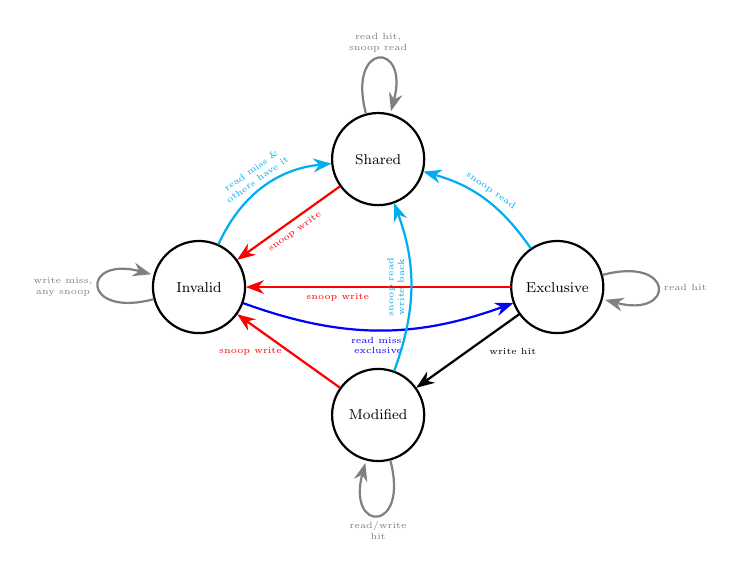
\begin{tikzpicture}[scale=0.65, transform shape,
    state/.style={circle, draw, minimum size=1.8cm, thick, font=\footnotesize},
    arrow/.style={->, >=Stealth, thick},
    %every edge/.style={arrow},
    auto,
    node distance=3.5cm
]

% Define states - closer together
\node[state] (invalid) at (0,0) {Invalid};
\node[state] (shared) at (3.5,2.5) {Shared};
\node[state] (exclusive) at (7,0) {Exclusive};
\node[state] (modified) at (3.5,-2.5) {Modified};

% Self-loops - only one per state
\path[arrow]
    (invalid) edge[loop left, gray]node[font=\tiny, left, align=center] {write miss,\\any snoop} (invalid)
    (shared) edge[loop above, gray] node[font=\tiny, text width=1.5cm, align=center] {read hit,\\snoop read} (shared)
    (exclusive) edge[loop right, gray] node[font=\tiny] {read hit} (exclusive)
    (modified) edge[loop below, gray] node[font=\tiny, text width=1.5cm, align=center] {read/write\\hit} (modified);

% Transitions between states - all unidirectional with better separation
\path[arrow]
    % From Invalid
    (invalid) edge[bend left=30, cyan] node[font=\tiny, above, sloped, text width=2cm, align=center] {read miss \&\\others have it} (shared)
    (invalid) edge[bend right=20, blue] node[font=\tiny, below, sloped, text width=1.8cm, align=center] {read miss,\\exclusive} (exclusive)
    
    % From Shared  
    (shared) edge[red] node[font=\tiny, below, sloped] {snoop write} (invalid)
%    (shared) edge[bend right=20, black] node[font=\tiny, below, sloped] {write hit} (exclusive)
    
    % From Exclusive  
    (exclusive) edge[bend right=20, cyan] node[font=\tiny, above, sloped] {snoop read} (shared)
    (exclusive) edge[black] node[font=\tiny, right, text width=1.5cm, align=center] {write hit} (modified)
    (exclusive) edge[red] node[font=\tiny, below, text width=2.8cm, align=left] {snoop write} (invalid)
    
    % From Modified
    (modified) edge[bend right=20, cyan] node[font=\tiny, above, sloped, text width=2cm, align=center] {snoop read\\write back} (shared)
    (modified) edge[red] node[font=\tiny, left] {snoop write} (invalid);

\end{tikzpicture}

\end{frame}


\begin{frame}{Multi-processor System: Inclusion}
  \begin{itemize}
    \item \textbf{L2 needs to keep track of the presence of each line in each of the processors}
    \begin{itemize}
      \item Determine if it needs to send a snoop to a processor
      \item Determine in what state to provide a requested line (S,E)
      \item[$\Rightarrow$] Need to guarantee that the L1 caches in each processor are inclusive of the L2 cache
    \end{itemize}
    \vspace{0.2cm}
    \item \textbf{When L2 evicts a line}
    \begin{itemize}
      \item L2 sends a snoop invalidate to all processors that have it
      \item If the line is modified in the L1 cache of one of the processors (in which case it exist only in that processor)
      \begin{itemize}
        \item The processor responds by sending the updated value to L2
        \item When the line is evicted from L2, the updated value gets written to memory
      \end{itemize}
    \end{itemize}
  \end{itemize}
\end{frame}

\begin{frame}{Global Observation (GO)}
\begin{itemize}
  \item A write is \textbf{globally observed} when any subsequent read by any processor returns its value
  \item Data for an RFO can be sent early, but GO cannot be granted until invalidations complete
  \item Prevents ordering violations where other cores still use stale values
\end{itemize}
\end{frame}

\begin{frame}{Inclusion vs. Non-Inclusive Designs}
\begin{itemize}
  \item Inclusive L2 is simple but wastes space when L2 is not much larger than L1
  \item \textbf{Non-inclusive} design: a separate \textbf{snoop filter} (tags + per-core valid bits) tracks sharers
  \item L1 and L2 can be mutually exclusive; L2 acts as a victim cache for L1
\end{itemize}
\end{frame}

\begin{frame}{Cache Optimization Summary}
\begin{center}
\footnotesize
\begin{tabular}{lccc}
\toprule
\textbf{Technique} & \textbf{Miss Rate} & \textbf{Miss Penalty} & \textbf{Hit Time}\\
\midrule
\textbf{Miss Rate Reduction:} & & & \\
\quad Larger Block Size & + & -- & \\
\quad Higher Associativity & + & & -- \\
\quad Victim Caches & + & & \\
\quad Pseudo-Associative Caches & + & & \\
\quad HW Prefetching of Instr/Data & + & & \\
\quad Compiler Controlled Prefetching & + & & \\
\quad Compiler Reduce Misses & + & & \\
\midrule
\textbf{Miss Penalty Reduction:} & & & \\
\quad Priority to Read Misses & & + & \\
\quad Sub-block Placement & & + & + \\
\quad Early Restart \& Critical Word 1st & & + & \\
\quad Non-Blocking Caches & & + & \\
\quad Second Level Caches & & + & \\
\bottomrule
\end{tabular}
\end{center}
\end{frame}

\begin{frame}{x86 Memory Ordering: Rules}
\begin{enumerate}
  \item Loads are not reordered with other loads.
  \item Stores are not reordered with other stores.
  \item Stores are not reordered with older loads.
  \item Loads may reorder with older stores to \emph{different} locations, but not to the same location.
  \item Causality respected; stores to the same location have a total order.
  \item Locked instructions are totally ordered and not reordered with loads/stores.
\end{enumerate}
\end{frame}

\begin{frame}[fragile]{x86 Ordering: Examples (1)}
\textbf{Loads and stores keep their own order}\\[3pt]
Initial: \texttt{x=y=0}. The outcome \texttt{r1=1, r2=0} is \textbf{not} allowed.
\begin{columns}[T]
\column{0.48\textwidth}
\textbf{Processor 0}
\begin{lstlisting}[basicstyle=\ttfamily\small]
Store [X] <- 1   // S1
Store [Y] <- 1   // S2
\end{lstlisting}
\column{0.48\textwidth}
\textbf{Processor 1}
\begin{lstlisting}[basicstyle=\ttfamily\small]
r1 <- Load [Y]   // L1
r2 <- Load [X]   // L2
\end{lstlisting}
\end{columns}
\end{frame}

\begin{frame}[fragile]{x86 Ordering: Examples (2)}
\textbf{Stores are not reordered with older loads}\\[3pt]
Initial: \texttt{x=y=0}. The outcome \texttt{r1=1, r2=1} is \textbf{not} allowed.
\begin{columns}[T]
\column{0.48\textwidth}
\textbf{Processor 0}
\begin{lstlisting}[basicstyle=\ttfamily\small]
r1 <- Load [X]   // L1
Store [Y] <- 1   // S1
\end{lstlisting}
\column{0.48\textwidth}
\textbf{Processor 1}
\begin{lstlisting}[basicstyle=\ttfamily\small]
r2 <- Load [Y]   // L2
Store [X] <- 1   // S2
\end{lstlisting}
\end{columns}
\end{frame}

\begin{frame}[fragile]{x86 Ordering: Examples (3)}
\textbf{Loads may reorder with older stores to different locations}\\[3pt]
Initial: \texttt{x=y=0}. Outcome \texttt{r1=0, r2=0} is \textbf{allowed}.
\begin{columns}[T]
\column{0.48\textwidth}
\textbf{Processor 0}
\begin{lstlisting}[basicstyle=\ttfamily\small]
Store [X] <- 1   // S1
r1 <- Load [Y]   // L1
\end{lstlisting}
\column{0.48\textwidth}
\textbf{Processor 1}
\begin{lstlisting}[basicstyle=\ttfamily\small]
Store [Y] <- 1   // S2
r2 <- Load [X]   // L2
\end{lstlisting}
\end{columns}
\end{frame}

\begin{frame}[fragile]{x86 Ordering: Examples (4)}
\textbf{Causality / transitive visibility}\\[3pt]
Initial: \texttt{x=y=0}. Outcome \texttt{r1=1, r2=1, r3=0} is \textbf{not} allowed.
\begin{columns}[T]
\column{0.32\textwidth}
\textbf{P0}
\begin{lstlisting}[basicstyle=\ttfamily\small]
Store [X] <- 1   // S1
\end{lstlisting}
\column{0.32\textwidth}
\textbf{P1}
\begin{lstlisting}[basicstyle=\ttfamily\small]
r1 <- Load [X]   // L1
Store [Y] <- 1   // S2
r2 <- Load [Y]   // L2
\end{lstlisting}
\column{0.32\textwidth}
\textbf{P2}
\begin{lstlisting}[basicstyle=\ttfamily\small]
r3 <- Load [X]   // L3
\end{lstlisting}
\end{columns}
\end{frame}

\begin{frame}{Slides intentionally omitted}
The original deck includes several figure-heavy slides (plots, bitfields, detailed
coherence transactions, PLRU trees). Per instructions, these have been summarized
or omitted here for Beamer. Consider adding vector (SVG/TikZ) figures later.
\end{frame}

\end{document}